\documentclass[10pt,a4paper,twoside,twocolumn]{article}
\usepackage[bg-a4, bg-print]{dnd} % Options: bg-a4, bg-letter, bg-full, bg-print, bg-none.
%\usepackage[bg-a4, bg-full]{dnd} % Options: bg-a4, bg-letter, bg-full, bg-print, bg-none.
\usepackage{xcolor}
\usepackage[italian]{babel} % Trennungsregeln und autom. Überschriften in n. dt. RS
\usepackage[utf8]{inputenc}
\usepackage{color}
\usepackage{esvect}
\usepackage{multirow}
\usepackage{graphicx}
\usepackage[binary-units]{siunitx} %unità di misura
\usepackage{amsfonts, amssymb}
\usepackage{mathtools}
\usepackage{booktabs} 
\usepackage{url}
\usepackage{circuitikz} % package to draw circuits
%\usepackage{hyperref} % url and hiperlinking
% Start document
\usepackage{hyperref}


\newcommand{\hfrac}{\rule[-1ex]{0ex}{3.5ex}} % altezza frazione

\definecolor{darkgreen}{rgb}{0,0.5,0}
\definecolor{orange}{rgb}{1,0.5,0}
\definecolor{purple}{rgb}{0.75,0,0.75}
\newtheorem{eserc}{Esercizio}[section]
\newtheorem{probl}{Problema}[section]


\begin{document}
\fontfamily{ppl}\selectfont % Set text font
\title{Lezione 7}
% Your content goes here

\section{Lezione 7}

\vspace{.3cm}



%     \item 17,18 maggio 
%       \begin{itemize}
%       \item 
%       \end{itemize}
%     \item 24,25 maggio (laboratorio aperto – non obbligatorio)
% 	\end{enumerate}
% \end{commentbox}

%Possibili box grafici: paperbox, subsection, quotebox, commentbox
\begin{paperbox}{Lezione di oggi e domani}
\begin{itemize}
\item Transistori BJT utilizzati con interruttori
\item Porte logiche elementari
\item Breve accenno su transistori MOS, FPGA e Microcontrollori
\end{itemize}
\end{paperbox}

Il transistore bipolare a  giunzione o
{\bf\color{red}BJT \color{black}} (\color{red}B\color{black}ipolar \color{red}J\color{black}unction \color{red}T\color{black}ransistor)
\`e un dispositivo a semiconduttore costituito da \emph{due} giunzioni p-n poste a distanza molto ravvicinata.

Pu\`o essere usato come \emph{amplificatore}; ad esempio nell'amplificatore operazionale 741 gli elementi attivi sono BJT.

Pu\`o anche essere usato come \emph{interruttore} nei circuiti digitali.


\subsection{Struttura del transistore bipolare a giunzione}
Il BJT \`e costituito da \textbf{DUE} giunzioni p-n 
separate da una distanza \textbf{minore} della lunghezza 
di diffusione dei portatori minoritari nella regione intermedia: 
$x_B < L_p$ per un transistore PNP (oppure $x_B < L_n$ per un transistore NPN)
\begin{figure}[h]
\centering
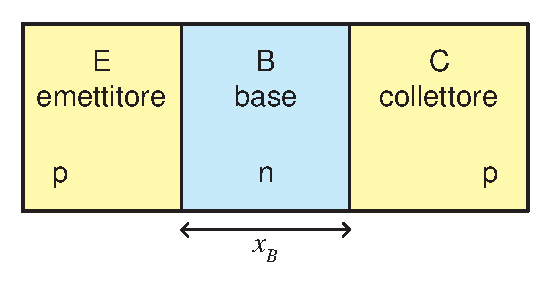
\includegraphics[width=0.6\columnwidth]{bjt1.eps}
\caption{Struttura del BJT}
\label{bjt1}
\end{figure}

Pu\`o essere di tipo \textbf{pnp} (come nella figura \ref{bjt1}) oppure \textbf{npn}.


Il BJT ha tre terminali:
\begin{itemize}
 \item E = emettitore (\emph{emitter})
\item B = base (\emph{base})
\item C = collettore (\emph{collector})
\end{itemize}
La base B \`e sempre drogata in modo opposto a collettore ed emettitore.

Quando la \textbf{giunzione E-B} \`e polarizzata \textbf{direttamente}
e la \textbf{giunzione C-B} \`e polarizzata \textbf{inversamente} 
si ha l'\textbf{effetto transistor} (Figura \ref{bjt3}).
\begin{figure}[h]
\centering
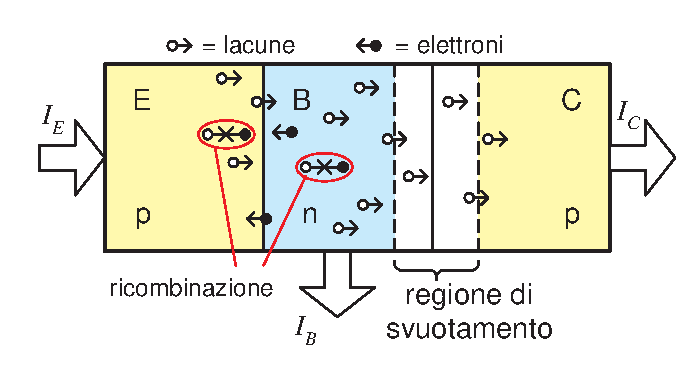
\includegraphics[width=0.7\columnwidth]{bjt3.eps}
\caption{Effetto transistor}
\label{bjt3}
\end{figure}

Attraverso la giunzione E-B, polarizzata direttamente, si verifica iniezione di portatori: in questo caso, le lacune vengono iniettate dall'emettitore nella base, e gli elettroni dalla base verso l'emettitore.

La base sottile ($x_B \ll L_p$) viene attraversata dalla maggior parte delle lacune iniettate, 
che muovendosi per diffusione nella base, raggiunge 
la giunzione di collettore \textbf{senza ricombinarsi}.

Nella giunzione C-B, polarizzata inversamente, c'e`un campo elettrico. Quando le lacune raggiungono la regione di svuotamento, le lacune vengono accelerate verso C dal campo elettrico (si muovono per deriva).


Un buon transistore deve avere due caratteritiche:
\begin{itemize}
\item %~\!\!\!
\color{red}
EMETTITORE PI\`U DROGATO DELLA BASE\color{black},
per avere una corrente dovuta quasi esclusivamente ai portatori iniettati dall'emettitore
(lacune per un transistore pnp; elettroni per un transistore npn);
\item %~\!\!\!
\color{red}
BASE SOTTILE rispetto alla lunghezza di diffusione\color{black},
per avere poca ricombinazione di portatori nella base.
\end{itemize}

Quando la giunzione E-B \`e polarizzata direttamente e la giunzione C-B \`e polarizzata inversamente
diciamo che il transistore lavora in \textbf{regione attiva}.
In questa condizione,
\textbf{quasi tutti i portatori iniettati dall'emettitore attraversano la base 
senza ricombinarsi e vengono raccolti dal collettore}.
La relazione tra le correnti (con i versi indicati nella figura \ref{bjt3}) \`e:
\begin{equation}
I_C = \alpha I_E
\label{alpha} 
\end{equation}
con $\alpha$ quasi uguale a 1 (ma $\alpha < 1$ perch\'e essendo la giunzione E-B polarizzata direttamente abbiamo $I_B > 0$).

Inoltre, la KCL applicata al `supernodo' costituito da tutto il BJT si pu\`o scrivere:
\begin{equation}
I_E = I_C + I_B
\label{kcl}
\end{equation}
e combinando le due equazioni precedenti si ricava
\begin{equation}
I_B = (1 - \alpha)I_E
\label{alpha1} 
\end{equation}
Poich\'e $\alpha$ \`e quasi uguale a 1, di solito in regione attiva $I_B$ \`e trascurabile.



\subsubsection{Simbolo del transistore bipolare}
\begin{figure}[h]
\centering
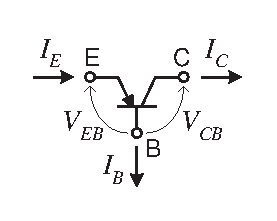
\includegraphics[width=0.35\columnwidth]{pnp1.eps}
~~~
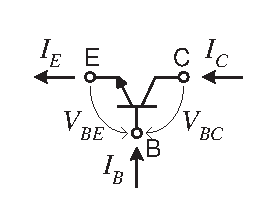
\includegraphics[width=0.35\columnwidth]{npn1.eps}
\caption{Simboli di transistori bipolari PNP (a sinistra) e NPN (a destra)}
\label{simboli}
\end{figure}
La figura \ref{simboli} illustra  i simboli dei due tipi di transistori.
Per ciascuno, sono indicati i versi convenzionali di correnti e tensioni, come verranno usati in seguito.

Si noti che nel simbolo la freccia indica il terminale di emettitore (E) ed \`e diretta dalla regione p verso la regione n (come nel diodo).
La corrente $I_E$ \`e concorde con il verso della freccia nel simbolo; i versi delle altre due correnti vengono presi in modo da avere sempre 
$I_E = I_C + I_B$.
In questo modo, in regione attiva tutte le correnti sono positive.



\subsection{Guadagno di corrente del transistore bipolare a  giunzione}
Combinando le tre equazioni \eqref{alpha}, \eqref{kcl} e \eqref{alpha1}, si ricava la relazione tra le correnti di collettore e di base:
\begin{equation}
I_C = \frac{\alpha}{1 - \alpha} I_B = \beta I_B
\label{beta} 
\end{equation}
dove
$\beta$ \`e il \textbf{guadagno di corrente}.
Normalmente, $\beta \gg 1$.
Ad esempio, se $\alpha = 0.99$, $\beta \approx 100$.

Il transistore bipolare \textbf{polarizzato in regione attiva} 
(giunzione E-B in diretta, giunzione C-B in inversa) 
si comporta da \textbf{amplificatore di corrente} 
(generatore di corrente controllato in corrente).
\begin{itemize}
\item
La corrente di ingresso \`e la corrente di base $I_B$
\item
La corrente di uscita \`e la corrente di collettore $I_C$
\item
Il guadagno di corrente \`e $\beta$:
\[
\beta = \frac{\alpha}{1 - \alpha} \approx \frac{1}{1 - \alpha} \text{~ (se~} \alpha \approx 1)
\]
\end{itemize}



\subsection{Regioni di funzionamento del transistore bipolare a  giunzione}
La tabella \ref{funz} riassume i quattro modi possibili di funzionamento del BJT.
\begin{table}
\begin{center}
\caption{Regioni di funzionamento del BJT}
\label{funz}
\begin{tabular}{|p{1.6cm}|p{1.7cm}||p{3.3cm}}
\textbf{giunzione E-B} & \textbf{giunzione C-B} & \textbf{funzionamento} \hfrac \\  
inversa & inversa & interdizione (spento, \emph{``off''}) \hfrac \\ 
diretta & inversa & regione attiva (diretta) \hfrac \\ 
diretta & diretta & saturazione \hfrac \\ 
inversa & diretta & regione attiva (inversa) \hfrac \\ 
\end{tabular}
\end{center}
\end{table}

Nei circuiti logici (digitali), il transistor viene usato come interruttore, facendolo lavorare tra spegnimento e saturazione.

Quando il transistore \`e in \textbf{interdizione (spento)}, le correnti sono nulle:
\[
I_B = I_C = I_E = 0
\]
e il BJT si comporta come un circuito aperto (interruttore spento).

Quando il BJT lavora in  \textbf{saturazione}, entrambe le giunzioni sono polarizzate direttamente.
Indicando il potenziale di giunzione con $V_\gamma$ (che per il silicio \`e $\approx 0.7$~V), possiamo scrivere:
\[
V_{EB} = V_\gamma; V_{CB} = V_\gamma
\]
e quindi la differenza di potenziale tra collettore ed emettitore \`e:
\[
V_{CE} \approx 0
\]
(non  \`e esattamente zero, perch\'e il potenziale dipende dal drogaggio e l'emettitore \`e pi\`u drogato, quindi la $V_\gamma$ per l'emettitore \`e leggermente maggiore della $V_\gamma$ del collettore).
In prima approssimazione, il BJT in saturazione pu\`o essere considerato come un cortocircuito (interruttore acceso) tra C ed E.

In \textbf{regione attiva}, invece, il BJT \`e un amplificatore di corrente con guadagno $\beta$:
\[
I_C = \beta I_B
\]
e
\[
V_{EB} = V_\gamma
\]
Usando resistenze, \` e possibile convertire la tensione in corrente e viceversa, ottenendo amplificatori di tensione (ad esempio, l'amplificatore operazionale 741 usa al suo interno qualche decina di BJT in regione attiva, e resistenze).

Di solito, la regione attiva inversa non viene usata, perch\'e il BJT funziona peggio.
Infatti, nonostante l'apparente simmetria della struttura, il drogaggio \emph{non} \`e simmetrico.
In regione attiva inversa, il collettore viene usato come emettitore e viceversa; tuttavia il collettore, non essendo molto drogato, ha un'efficienza pi\`u bassa e il guadagno di corrente \`e molto minore.



\subsection{Logica RTL}
La logica RTL (Resistor-Transistor Logic), come indica il nome, fa uso di transistori e resistenze.
\begin{figure}[t]
\centering
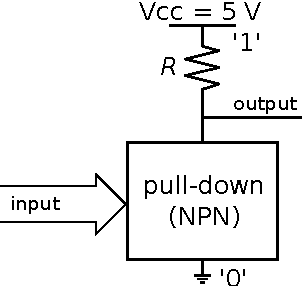
\includegraphics[width=0.4\columnwidth]{logic1.pdf}
\caption{Logica RTL}
\label{logic1}
\end{figure}

La figura \ref{logic1} rappresenta la struttura generale di una porta logica RTL che fa uso di transistori bipolari NPN. La parte con i transistori NPN, il cui schema dipende dalla funzione logica che il circuito deve realizzare, si chiama ``pull-down'' perch\'e la sua accensione porta a zero l'uscita.
La resistenza $R$ costituisce il ``pull-up''; quando il pull-down \`e spento, la corrente nel circuito va a zero e la resistenza porta l'uscita al valore alto ($+V_{CC}$).


\subsection{Inverter RTL}
\begin{figure}[t]
\centering
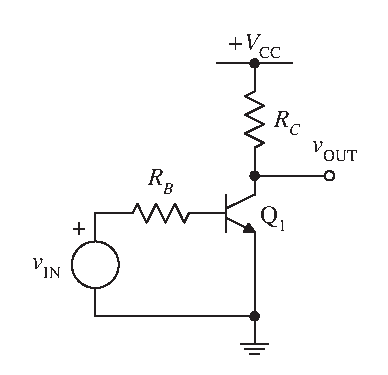
\includegraphics[width=0.5\columnwidth]{npn_inv.eps}
\caption{Inverter RTL}
\label{npn_inv}
\end{figure}
La figura \ref{npn_inv} illustra un inverter (porta logica ``NOT'') in tecnologia RTL.

Il transistore Q$_1$ ha una tensione di accensione $V_\gamma = 0.7 \text{~V}$, e un guadagno di corrente $\beta = 200$ in regione attiva.
La tensione di alimentazione \`e
$V_\text{CC} = 5 \text{~V}$; le resistenze sono $R_{C} = 2.2\text{~k}\Omega$ e  $R_{B} = 22 \text{~k}\Omega$.
Il segnale di ingresso  $v_\text{IN}$ \`e un'onda quadra a frequenza relativamente bassa (dell'ordine del kilohertz) con valore basso 0~V e valore alto 5~V. 
Vogliamo studiare il funzionamento del circuito.

Anzitutto, attribuiamo un valore logico, cio\`e binario, ai valori di tensione.
In altre parole, ci interessa solo l'informazione a due valori (alto/basso, vero/falso);
questi due livelli corrispondono ai valori binari `1' e `0'.
Una grandezza in cui osserviamo solo il livello (alto o basso) codifica un \textbf{bit} di informazione (\textbf{bit} = \textbf{bi}nary dig\textbf{it}, cio\`e una cifra nel sistema di numerazione in base 2).
In \emph{logica positiva}, la tensione alta corrisponde al bit `1', mentre la tensione bassa corrisponde al bit `0'.


Analizziamo dapprima il caso in cui $v_\text{IN} = 0 \text{~V}$.
Nella maglia di ingresso il generatore \`e spento; quindi nella resistenza $R_B$ non pu\`o scorrere corrente.
Siccome la corrente di base \`e nulla,
Q$_1$ \`e spento e abbiamo $I_B = I_C = I_E = 0$. 
Nel circuito non passa corrente; 
$V_B = 0$ e $V_C = V_\text{CC} = 5 \text{~V}$.
Di conseguenza,
la tensione di uscita \`e $v_\text{OUT} = V_C = 5 \text{~V}$.


Consideriamo ora il caso $v_\text{IN} = 5 \text{~V}$.
Anzitutto, osserviamo che nella maglia di ingresso abbiamo una differenza di tensione maggiore del potenziale di giunzione, e quindi la giunzione B-E di Q$_1$ \`e polarizzata direttamente; ne consegue che Q$_1$ \`e acceso (pu\`o essere in regione attiva oppure in saturazione).
In ogni caso, al nodo di base la tensione \`e $V_B = 0.7 \text{~V}$ e 
la corrente \`e $I_B = \frac{V_{in} - V_B}{R_B} \approx 0.2 \text{~mA}$.

Se Q$_1$ fosse in regione attiva, la corrente di collettore dovrebbe essere $I_C = \beta I_B \approx 4.4 \text{~mA}$ e la caduta di tensione sulla resistenza $R_C$

Q$_1$ in saturazione\color{black}: $V_{BE} = V_{BC} = V_\gamma = 0.7 \text{~V}$. 
\begin{itemize}
\item
$V_B = 0.7 \text{~V}$; 
\item
$V_C = 0$; 
\item
$I_B = \frac{V_{in} - V_B}{R_B} = 0.43 \text{~mA}$; 
\item
$I_C = \frac{V_\text{CC} - V_C}{R_C} = 5 \text{~mA}$. 
\end{itemize}
La tensione di uscita \`e $v_\text{OUT} = V_C = 0$.



Se i valori di tensione $0$ e $5  \text{~V}$ 
corrispondono rispettivamente ai bit ``0'' e ``1'', 
possiamo riepilogare il funzionamento del circuito con la tabella
\\
(X = bit di ingresso; Y = bit di uscita)
\begin{center}
\begin{tabular}{|c|c||c||c|c|} 
X & $v_\text{IN}$ & Q$_1$ & $v_\text{OUT}$ & Y \hfrac \\ 
0 & $0 \text{~V}$ & interdizione (``off'') & $5 \text{~V}$ & 1 \hfrac \\
1 & $5 \text{~V}$ & saturazione & $0 \text{~V}$ & 0 \hfrac \\ 
\end{tabular}
\end{center}
Leggendo la prima e l'ultima colonna, si ricava che il circuito 
realizza la funzione di una porta logica \textbf{NOT} (inverter):
\begin{center} \leavevmode
%\includegraphics[width=0.4\columnwidth]{inv.eps}
\end{center}

\subsection{Segnali digitali e funzioni logiche}
\begin{itemize}
\item
SEGNALE DIGITALE: variabile elettrica (di solito una tensione) 
a cui vengono associati solamente due possibili valori
\begin{itemize}
\item
1 = Alto = Vero
\item
0 = Basso = Falso
\end{itemize}
\item
FUNZIONE LOGICA: funzione i cui ingressi e uscite sono segnali digitali
\bigskip

\item 
I segnali digitali tollerano inaccuratezze dei componenti e rumore
\item
Le funzioni logiche sono semplici e ripetitive
\item
La progettazione digitale \`e automatizzata
\end{itemize}



\subsection{Domini di rappresentazione (1/2)}
Qualsiasi sistema elettronico pu\`o essere rappresentato in pi\`u modi, 
usando differenti linguaggi, ciascuno dei quali serve a descrivere alcune 
delle caratterestiche del sistema.

I domini di rappresentazione pi\`u frequentemente usati sono:
\begin{itemize}
\item \textbf{\color{darkgreen}dominio comportamentale}: descrive le relazioni ingresso-uscita tra i segnali;
\item \textbf{\color{blue}dominio strutturale}: descrive la suddivisione in parti e le interconnessioni;
\item \textbf{\color{red}dominio fisico}: descrive l'ingombro fisico e i materiali.
\end{itemize}



\subsection{Domini di rappresentazione (2/2)}
\vspace{-5mm}
\begin{center}
\epsfxsize = 0.75 \columnwidth
\epsfbox{domini.eps}
\end{center}



\subsection{Livelli di astrazione}
In ciascun dominio, la rappresentazione del sistema pu\`o essere fatta a
\color{red} \textbf{diversi livelli di astrazione}\color{black}.

\begin{itemize}
\item 
I livelli di maggiore dettaglio sono adeguati per la descrizione 
di sottosistemi semplici.
\item 
Per la rappresentazione di sistemi molto complessi occorre ricorrere 
ad un maggiore livello di astrazione: 
nella descrizione si considerano solo gli aspetti essenziali e 
si tralasciano gli aspetti di dettaglio che non sono rilevanti per la descrizione 
del sistema nel suo complesso.
\end{itemize}



\subsection{Legge di Moore (1/2)}
\textbf{Legge di Moore} (1965):
\begin{itemize}
\item \color{red}
Il numero di transistori integrati su un chip, a parit\`a di area di silicio, 
raddoppia ogni 18 mesi circa.\color{black}
\end{itemize}
\emph{Nota: nel 1965 il circuito integrato pi\`u complesso aveva solo 64 transistori!}

Oggi, la legge di Moore \`e usata per pianificare le modifiche 
alla tecnologia di fabbricazione.
\vspace{5mm}

\hrule
\vspace{3mm}

{\footnotesize
G.E.~Moore, ''Cramming more components onto integrated circuits'', \emph{Electronics}, Volume 38, Number 8, April 19, 1965.
}



\subsection{Legge di Moore (2/2)}
Una delle previsioni contenute nell'articolo di Gordon Moore (1965):
\begin{center}
\epsfxsize = \columnwidth
\epsfbox{moore.eps}
\end{center}
\vspace{5mm}

\hrule
\vspace{3mm}

{\footnotesize
G.E.~Moore, ''Cramming more components onto integrated circuits'', \emph{Electronics}, Volume 38, Number 8, April 19, 1965.
}



\subsection{Evoluzione delle tecniche di progetto}
La Legge di Moore ha richiesto continui cambiamenti: 
\begin{itemize}
\item nella tecnologia di fabbricazione di circuiti integrati;
\item nelle tecniche di progettazione;
\item nelle metodologie di collaudo.
\end{itemize}
Il concetto di ``sistema'' ha subito, nel tempo, un'analoga evoluzione:
\begin{itemize}
\item 1980: nasce il VLSI (Very Large Scale Integration) --- un milione di transistori su un solo chip;
\item oggi: Giga-Scale Integration --- oltre un miliardo di transistori su un chip.
\end{itemize}




\subsection{Criteri generali (1/2)}
Un buon progetto deve seguire alcune regole:
\begin{itemize}
\item 
\textbf{Gerarchia}: un sistema complesso deve essere scomposto in sottosistemi, 
e il procedimento di scomposizione deve essere iterato fino a che il progetto del singolo blocco pu\`o essere fatto da un solo progettista.
\item 
\textbf{Regolarit\`a}: i vari blocchi devono avere caratteristiche ``simili'', 
che ne facilitino l'assemblaggio nel sistema completo.
\end{itemize}



\subsection{Criteri generali (2/2)}
\begin{itemize}
\item 
\textbf{Modularit\`a}: quando \`e possibile, \`e opportuno utilizzare il minor numero possibile di blocchi differenti. Inoltre, \`e opportuno che tutti i blocchi abbiano
interfacce standard.
\item
\textbf{Localizzazione dei segnali}: tutto ci\`o che non costituisce elemento di interfaccia verso l'esterno di un blocco, deve essere localizzato all'interno del blocco stesso.
\end{itemize}



\subsection{Esempio: inverter (1/3)}
\begin{center}
\epsfxsize = 0.45 \columnwidth
\epsfbox{inv_sym.eps}
\end{center}
Rappresentazione comportamentale:
\begin{itemize}
\item
Funzione booleana:
\[ Y = \overline{A} ~~~\text{oppure}~~~ Y = \textrm{not}(A) \]
\item
Tabella della verit\`a:
\begin{center}
\begin{tabular}{|c||c|}
\hline
$A$ & $Y$ \\ \hline
\hline
$0$ & $1$ \\ \hline
$1$ & $0$ \\ \hline
\end{tabular}
\end{center}
\end{itemize}



\subsection{Esempio: inverter (2/3)}
Rappresentazione strutturale:
\vspace{-10mm}
\begin{center}
\begin{tabular}{c c}
\epsfxsize = 0.35 \columnwidth \epsfbox{inv_sym.eps}
&
\epsfxsize = 0.3 \columnwidth \epsfbox{inv_schema.eps}
\\
Simbolo
&
Schema
\\
\end{tabular}
\end{center}
Netlist:
\begin{verbatim}
.SUBCKT INV in out vdd vss
MP out in vdd vdd PMOS 
MN out in vss vss NMOS
.ENDS INV
\end{verbatim}



\subsection{Esempio: inverter (3/3)}
Rappresentazione \\
fisica \\
(layout):
\vspace{-20mm}
\begin{center}
\begin{tabular}{c}
\epsfxsize = 0.3 \columnwidth \epsfbox{inv_lay.eps}
\end{tabular}
\end{center}



\subsection{Descrizione fisica}
La descrizione fisica \`e costituita da un insieme di forme geometriche definite 
in coordinate cartesiane (piano $xy$).

Ogni geometria appartiene ad un determinato ``layer'', cio\`e strato di materiale.
I layer sono disposti uno sopra l'altro (lungo l'asse $z$):
well, diffusione N e diffusione P, polisilicio, contatto, metallizzazione.

\bigskip

Linguaggi per la descrizione fisica:
\begin{itemize}
\item
CIF (Caltech Intermediate Form): formato testo

{\footnotesize Una descrizione del CIF si trova in: C. Mead and L. Conway, 
\emph{Introduction to VLSI Systems.} Addison-Wesley, Reading, MA, USA, 1980.}

\item
GDS II: formato binario, pi\`u compatto, 
di fatto \`e lo standard usato nelle industrie di semiconduttori
\end{itemize}



\subsection{CIF (Caltech Intermediate Form)}
\vspace{-2mm}
\begin{verbatim}
DefStart 101; (inizio definizione oggetto 101)
Layer CNWell; (usa il layer N-Well)
Box 1500 1800 750 2100; (dimensioni e centro)
Layer CPDiff;
Box 1000 1200 800 2000;
Layer CNDiff;
Box 1000 600 800 700;
Layer CPoly;
Box 250 2000 800 1500;
Layer CCont;
...
Layer CMetal;
...
DefFinish; (fine definizione oggetto)
Call 101 Translate -500 1500 MirrorX; (istanza)
\end{verbatim}



\subsection{Porte logiche elementari}
\begin{itemize}
\item
Ad ogni FUNZIONE LOGICA elementare nel dominio
comportamentale corrisponde una PORTA LOGICA (o
``GATE'') nel dominio strutturale, la quale a sua volta pu\`o
avere diverse implementazioni circuitali.
\item
In TECNOLOGIA CMOS le porte logiche sono realizzate
con transistori MOS complementari (NMOS e PMOS)
realizzati su un unico substrato di silicio.
\end{itemize}



\subsection{Algebra di Boole (1/12)}
\begin{itemize}
\item
VALORI:
\begin{itemize}
\item
1 = Alto = Vero
\item
0 = Basso = Falso
\item
(ci sono estensioni a pi\`u di due valori)
\end{itemize}
\item
FUNZIONI ELEMENTARI:
\begin{itemize}
\item
NOT (negazione): \\
$y = \overline{a}$~~$\Longleftrightarrow$~~$y$ \`e vero se $a$ \`e falso, e viceversa
\begin{center}
\epsfxsize = 0.3 \columnwidth
\epsfbox{inv_sym.eps}
\end{center}
\item
AND (prodotto logico):
$y = a_1 \cdot a_2 \cdot \ldots \cdot a_n$
\item
OR (somma logica):
$y = a_1 + a_2 + \ldots + a_n$
\end{itemize}
\end{itemize}



\subsection{Algebra di Boole (2/12)}
\begin{itemize}
\item
FUNZIONI ELEMENTARI (continuazione):
\begin{itemize}
\item
NOT (negazione): $y = \overline{a}$
\item
AND (prodotto logico): 
$y = a_1 \cdot a_2 \cdot \ldots \cdot a_n$~~$\Longleftrightarrow$ \\ 
$y$ \`e vero se tutti gli $a_i$ sono veri, altrimenti \`e falso
\begin{center}
\epsfxsize = 0.3 \columnwidth
\epsfbox{andn_sym.eps}
\end{center}
\item
OR (somma logica): 
$y = a_1 + a_2 + \ldots + a_n$~~$\Longleftrightarrow$ \\
$y$ \`e falso se tutti gli $a_i$ sono falsi, altrimenti \`e vero
\begin{center}
\epsfxsize = 0.3 \columnwidth
\epsfbox{orn_sym.eps}
\end{center}
\end{itemize}
\end{itemize}



\subsection{Algebra di Boole (3/12)}
\begin{itemize}
\item
PROPRIET\`A FONDAMENTALI:
\begin{itemize}
\item
Idempotenza:

\raisebox{7mm}{$x + x = x$ ~~~~~~~~}
\epsfxsize = 0.6 \columnwidth
\epsfbox{or2xx_sch.eps}

~ \\

\raisebox{7mm}{$x \cdot x = x$ ~~~~~~~~~}
\epsfxsize = 0.6 \columnwidth
\epsfbox{and2xx_sch.eps}
\end{itemize}
\end{itemize}



\subsection{Algebra di Boole (4/12)}
\begin{itemize}
\item
PROPRIET\`A FONDAMENTALI (continuazione):
\begin{itemize}
\item
Propriet\`a commutativa:

\raisebox{7mm}{$x + y = y + x$ ~~~~~~~~}
\epsfxsize = 0.5 \columnwidth
\epsfbox{or2xy_sch.eps}

~ \\

\raisebox{7mm}{$x \cdot y = y \cdot x$ ~~~~~~~~~~}
\epsfxsize = 0.5 \columnwidth
\epsfbox{and2xy_sch.eps}
\end{itemize}
\end{itemize}



\subsection{Algebra di Boole (5/12)}
\begin{itemize}
\item
PROPRIET\`A FONDAMENTALI (continuazione):
\begin{itemize}
\item
Propriet\`a associativa:
\[(x + y) + z = x + (y + z)\]
\begin{center}
\epsfxsize = 0.8 \columnwidth
\epsfbox{or3xyz_sch.eps}
\end{center}
\vspace{3mm}
\[ (x \cdot y) \cdot z = x \cdot (y \cdot z)\]
\begin{center}
\epsfxsize = 0.78 \columnwidth
\epsfbox{and3xyz_sch.eps}
\end{center}
\end{itemize}
\end{itemize}



\subsection{Algebra di Boole (6/12)}
\begin{itemize}
\item
ALTRE PROPRIET\`A FONDAMENTALI:
\begin{itemize}
\item
Complementazione:

\raisebox{7mm}{$x + \overline{x} = 1$ ~~~~~~~~}
\epsfxsize = 0.6 \columnwidth
\epsfbox{or2xxn_sch.eps}

~ \\

\raisebox{7mm}{$x \cdot \overline{x} = 0$ ~~~~~~~~~}
\epsfxsize = 0.6 \columnwidth
\epsfbox{and2xxn_sch.eps}
\end{itemize}
\end{itemize}



\subsection{Algebra di Boole (7/12)}
\begin{itemize}
\item
ALTRE PROPRIET\`A FONDAMENTALI:
\begin{itemize}
\item
Propriet\`a distributiva (1):
\[ x \cdot (y + z) = x \cdot y + x \cdot z \]
\begin{center}
\epsfxsize = 0.8 \columnwidth
\epsfbox{andor3xyz_sch.eps}
\end{center}
\end{itemize}
\end{itemize}



\subsection{Algebra di Boole (8/12)}
\begin{itemize}
\item
ALTRE PROPRIET\`A FONDAMENTALI (continuazione):
\begin{itemize}
\item
Propriet\`a distributiva (2):
\[ x + (y \cdot z) = (x  + y) \cdot (x + z) \]
\begin{center}
\epsfxsize = 0.8 \columnwidth
\epsfbox{orand3xyz_sch.eps}
\end{center}
\end{itemize}
\end{itemize}



\subsection{Algebra di Boole (9/12)}
\begin{itemize}
\item
ALTRE PROPRIET\`A FONDAMENTALI (continuazione):
\begin{itemize}
\item
Ricorsivit\`a della negazione:
\[ \overline{\left(\overline{x}\right)} = x \]
\begin{center}
\epsfxsize = 0.7 \columnwidth
\epsfbox{xnn_sch.eps}
\end{center}
\end{itemize}
\end{itemize}



\subsection{Algebra di Boole (10/12)}
\begin{itemize}
\item
Propriet\`a di assorbimento (1):

\raisebox{7mm}{$x + 0 = x$ ~~~~~~~~}
\epsfxsize = 0.4 \columnwidth
\epsfbox{or2x0_sch.eps}
\vspace{2mm}

\raisebox{7mm}{$x \cdot 1 = x$ ~~~~~~~~~}
\epsfxsize = 0.4 \columnwidth
\epsfbox{and2x1_sch.eps}
\vspace{2mm}

\raisebox{7mm}{$ x + 1 = 1$ ~~~~~~~~}
\epsfxsize = 0.38 \columnwidth
\epsfbox{or2x1_sch.eps}
\vspace{2mm}

\raisebox{7mm}{$x \cdot 0 = 0$ ~~~~~~~~~}
\epsfxsize = 0.35 \columnwidth
\epsfbox{and2x0_sch.eps}
\end{itemize}



\subsection{Algebra di Boole (11/12)}
\begin{itemize}
\item
Propriet\`a di assorbimento (2):

\raisebox{7mm}{$x + x \cdot y = x$ ~~~~~~~~}
\epsfxsize = 0.5 \columnwidth
\epsfbox{orand3xxy_sch.eps}
\vspace{2mm}

\raisebox{7mm}{$x \cdot (x + y) = x$ ~~~~~~}
\epsfxsize = 0.5 \columnwidth
\epsfbox{andor3xxy_sch.eps}
\vspace{2mm}

\raisebox{7mm}{$x + \overline{x} \cdot y = x + y$ ~~~~}
\epsfxsize = 0.62 \columnwidth
\epsfbox{orand3xxny_sch.eps}
\vspace{2mm}

\raisebox{7mm}{$x \cdot (\overline{x} + y) = x \cdot y$ ~~~}
\epsfxsize = 0.62 \columnwidth
\epsfbox{andor3xxny_sch.eps}
\end{itemize}



\subsection{Algebra di Boole (12/12)}
\begin{itemize}
\item
TEOREMA DI DE MORGAN:
\vspace{2mm}

\raisebox{7mm}{$\overline{x + y} = \overline{x} \cdot \overline{y}$ ~~~~~~~}
\epsfxsize = 0.62 \columnwidth
\epsfbox{nor2demorgan_sch.eps}
\vspace{2mm}

\raisebox{7mm}{$\overline{x \cdot y} = \overline{x} + \overline{y}$ ~~~~~~~}
\epsfxsize = 0.62 \columnwidth
\epsfbox{nand2demorgan_sch.eps}
\vspace{2mm}

\item
DUALIT\`A:
\[ \overline{f} \left( x_1, x_2, \ldots, x_n, 0, 1, +, \cdot \right) = f \left( \overline{x_1}, \overline{x_2}, \ldots, \overline{x_n}, 1, 0, \cdot, + \right) \]
\end{itemize}



\subsection{Bibliografia}
Per un approfondimento sui domini di rappresentazione, si veda:
\begin{itemize}
\item
N.H.E.\ Weste and K. Eshraghian, \emph{Principles of CMOS VLSI Design: A Systems Perspective  (2nd edition)}. Addison-Wesley, Reading, MA, USA, 1993 -- Capitolo~1 e Paragrafo 6.2.

(Controllare a pagina iv del libro: deve essere la ristampa con correzioni dell'ottobre 1994, o con data successiva.)
\end{itemize}


\subsection{FPGA}

\subsection{Microcontrollori}


\begin{monsterbox}{Esercizi}
\begin{enumerate}
\item Trovare la caratteristica tensione-corrente per diversi diodi: diodo convenzionale, led rosso, led giallo, led verde.
\item 
\end{enumerate}
\end{monsterbox}



\end{document}
